%%%%%%%%%%%%%%%%%%%%%%%%%%%%%%%%%%%%%%%%%
% Imperial Placement Report Template
% LaTeX Template
% Version 1.0 (28/06/16)
%%%%%%%%%%%%%%%%%%%%%%%%%%%%%%%%%%%%%%%%%
%----------------------------------------------------------------------------------------
%	PACKAGES AND OTHER DOCUMENT CONFIGURATIONS
%----------------------------------------------------------------------------------------

\documentclass[a4paper,12pt,titlepage]{article}
\usepackage[left=3cm,right=3cm,top=3.5cm,bottom=3cm]{geometry}
\usepackage[english]{babel}
\usepackage[utf8x]{inputenc}
\usepackage{amsmath}
\usepackage{amsfonts}
\usepackage{graphicx}
\usepackage[colorinlistoftodos]{todonotes}
\usepackage[toc,page]{appendix}
\usepackage{fancyhdr}
\usepackage{listings}
\usepackage{color}

\definecolor{codegreen}{rgb}{0,0.6,0}
\definecolor{codegray}{rgb}{0.5,0.5,0.5}
\definecolor{codepurple}{rgb}{0.58,0,0.82}
\definecolor{backcolour}{rgb}{0.95,0.95,0.95}

\makeatletter
\def\BState{\State\hskip-\ALG@thistlm}
\makeatother

\pagestyle{fancy}
\fancyhf{}
\fancyhead[L]{\textit{\nouppercase{\rightmark}}}
\fancyhead[R]{\thepage}

\setlength{\parindent}{0em}
\renewcommand{\baselinestretch}{1.5}

\lstdefinestyle{mystyle}{
    backgroundcolor=\color{backcolour},
    commentstyle=\color{codegreen},
    keywordstyle=\color{magenta},
    numberstyle=\tiny\color{codegray},
    stringstyle=\color{codepurple},
    basicstyle=\footnotesize,
    breakatwhitespace=false,
    breaklines=true,
    captionpos=b,
    keepspaces=true,
    numbers=left,
    numbersep=5pt,
    showspaces=false,
    showstringspaces=false,
    showtabs=false,
    tabsize=2
}

\lstset{style=mystyle}

\begin{document}
\newcount\colveccount
\newcommand*\colvec[1]{
        \global\colveccount#1
        \begin{pmatrix}
        \colvecnext
}
\def\colvecnext#1{
        #1
        \global\advance\colveccount-1
        \ifnum\colveccount>0
                \\
                \expandafter\colvecnext
        \else
                \end{pmatrix}
        \fi
}

\begin{titlepage}

\newcommand{\HRule}{\rule{\linewidth}{0.5mm}} % Defines a new command for the horizontal lines, change thickness here
\setlength{\topmargin}{0in}
\center % Center everything on the page


%----------------------------------------------------------------------------------------
%	HEADING SECTIONS
%----------------------------------------------------------------------------------------

\textsc{\LARGE Imperial College London}\\[1.5cm] % Name of your university/college
\textsc{\Large Department of Computing}\\[0.5cm] % Major heading such as course name

%----------------------------------------------------------------------------------------
%	TITLE SECTION
%----------------------------------------------------------------------------------------

\HRule \\[0.4cm]
{ \huge \bfseries Drone Network Simulation\\on SpatialOS\\\textit{Interim Report}}\\[0.4cm] % Title of your document
\HRule \\[0.4cm]

%----------------------------------------------------------------------------------------
%	AUTHOR SECTION
%----------------------------------------------------------------------------------------

\begin{minipage}[t]{0.4\textwidth}
\begin{flushleft} \large
\emph{Author:}\\
Paul \textsc{Balaji} \\
\end{flushleft}
\end{minipage}
\begin{minipage}[t]{0.5\textwidth}
\begin{flushright} \large
\emph{Supervisor:} \\
Prof.~William \textsc{Knottenbelt}
\end{flushright}
\begin{flushright} \large
\emph{Second Marker:} \\
To.~Be \textsc{Decided}
\end{flushright}
\end{minipage}\\[1cm]

%----------------------------------------------------------------------------------------
%	DATE SECTION
%----------------------------------------------------------------------------------------

{\large \today}\\[0.5cm] % Date, change the \today to a set date if you want to be precise


\vfill % Fill the rest of the page with whitespace

\end{titlepage}

% \renewcommand{\abstractname}{\large Abstract}
% \begin{abstract}
% test post pls ignore
% \end{abstract}
%
% \renewcommand{\abstractname}{\large Acknowledgements}
% \begin{abstract}
% ack
% \end{abstract}

\newpage

\tableofcontents

\newpage

\section{Introduction}
Drone technology is becoming increasingly popular. Their agility and ability to be used remotely makes them ideal for a number of use cases in  numerous industries such as film, law enforcement, emergency services, agriculture and commercial delivery\cite{Koontz}. \\

Due to numerous advances in technology, drones are quickly advancing to the point where human input is no longer a necessity. This has led to many companies showing interest in integrating drones with their work in the coming years. \\

Although it may be an engineer's dream for a fully automated world, drones in particular are a harrowing reminder that there are real risks associated with them. There are already several incidents of drones crashing into planes and flying into areas they shouldn't, most notably near Heathrow airport\cite{BBCNews2017}. All of this provides motivation to introduce some form of autonomous air traffic control system to navigate these drones to their respective destinations in a safe manner.\\

However, prior work has been done on the routing and navigation aspect of such a system. In order for drones to truly take over more aspects of our lives, we must look at how they can provide a tangible cost-benefit to specific use-cases. There is no doubt that simply removing the human element can save costs drastically, and there is none more exciting a scenario than with deliveries. For example, Amazon stands to increase their margins considerably if they can successfully pull off their Prime Air initiative\cite{Welch2015}.

% delivery market stands to gain even more by optimising deliveries for profit / consider QoS

% the natural next step is to schedule / distribute the deliveries across network in addition to routing

% not advisable to test in production, so best port of call is to simulate

% many companies are investigating how to produce richer, meaningful simulations [cite improbable / SpatialOS]

% we have shown a new model of deliveries based on a QoS value curve

% show how net profit in a system changes depending on the type of scheduling mechanism used

\subsection{Autonomous Systems}
\subsection{Making Money}


%**********************************************%
\newpage
\section{Background}
We first provide an insight into drones, and the considerations to account for when applying them in day to day life. Additionally we summarise prior work completed by Imperial students on an autonomous air traffic control system. \\

We then continue to discuss modern delivery networks and introduce a mechanism by which economic value is prioritised. Finally, we give details about Improbable's SpatialOS and the reasoning for using this platform for the drone simulation.

\subsection{Drones}
As we have introduced, drones stand to be a revolutionary part of our lives as we welcome the new, incoming era of automation. However, to be practical there are a few key concepts one must understand to ensure that they remain a help and not a harm or hinderence to mankind.

\subsubsection{No Fly Zones}
No Fly Zones (which we will abbreviate as NFZs) are geographical areas where a drone is not allowed to enter or fly at any altitude. Examples of these may include Hyde Park, Buckingham Palace, airports and military locations. Typically these are static obstacles that will always remain a NFZ, however we could also consider cases when they could be created dynamically.\\

Suppose there was an issue of national security, it would be beneficial for the security and intelligence services to set up a temporary NFZ around areas where they deem a risk so that they can conduct their own operations without worry of external parties interfering with the situation.

\subsubsection{Manned Aviation}
Manned Aviation is any form of airborne transport with humans on board. This would include passenger jets, private jets, helicopters and other miscallaneous vechicles. For simulation purposes, we can consider these to have straight paths from a start to an end because relative to the zig-zagging of drones - they are effectively straight. \\

It is paramount to avoid collisions with manned aviation because there is a high risk of human calamity, in addition to the bad press and financial costs associated with such an air traffic incident.

\subsubsection{Other Drones}
Naturally we would want to make sure that we avoid colliding into other drones as well. In a perfect system, a single air traffic controller would have totalitarian dominance over all drones that take to the skies - however this is not \textit{Black Mirror} and we have to assume that there will always be drones that this system will not be able to control or predict. \\

Nonetheless, a system can ensure that it navigates drones under its control as best as it can, avoiding these external drones and other rogue drones that may be flying with the sole intention of causing problems to others.

\subsubsection{Toll Zones}
Toll Zones are geographical areas where a drone has to pay an extra fee to pass through at any altitude. It is a very similar idea to the one that led to Congestion Charges being applied to much of central London. By restricting certain areas only to those who are willing to pay the fee to use the airspace, it reduces the density of air traffic in a specific area. These charges could also be used as an incentive to reduce pollution in the toll zone, and the additional revenue generated by the toll fees could be used towards the drone-related systems in place within the zone.

\subsection{Autonomous Air Traffic Control (AATC)}
\subsubsection{What is AATC?}
During the Autumn Term of the 2016-17 academic year, several students undertook a group project in association with Microsoft and Altitude Angel to produce an autonomous air traffic control system. The goal of the project was to safely navigate drones from their start to their end goals, whilst avoiding obstacles and taking the shortest possible path to minimise battery use.

\subsubsection{Technical Overview}
AATC has a simple client-server architecture, where drones connect to the REST service to send their telemetry information and goal waypoints every second. The server sends back direction recommendations to navigate the drone to its destination. \\

Because it would have been too expensive to trial the system on actual drones, a test bench was also implemented that would simulate the drones polling the server and responding to its recommendations. This test bench produced a set of simulation data, that is then available to view on the AATC visualiser\cite{Balaji2017a}.

\begin{figure}[!hbpt]
  \center
  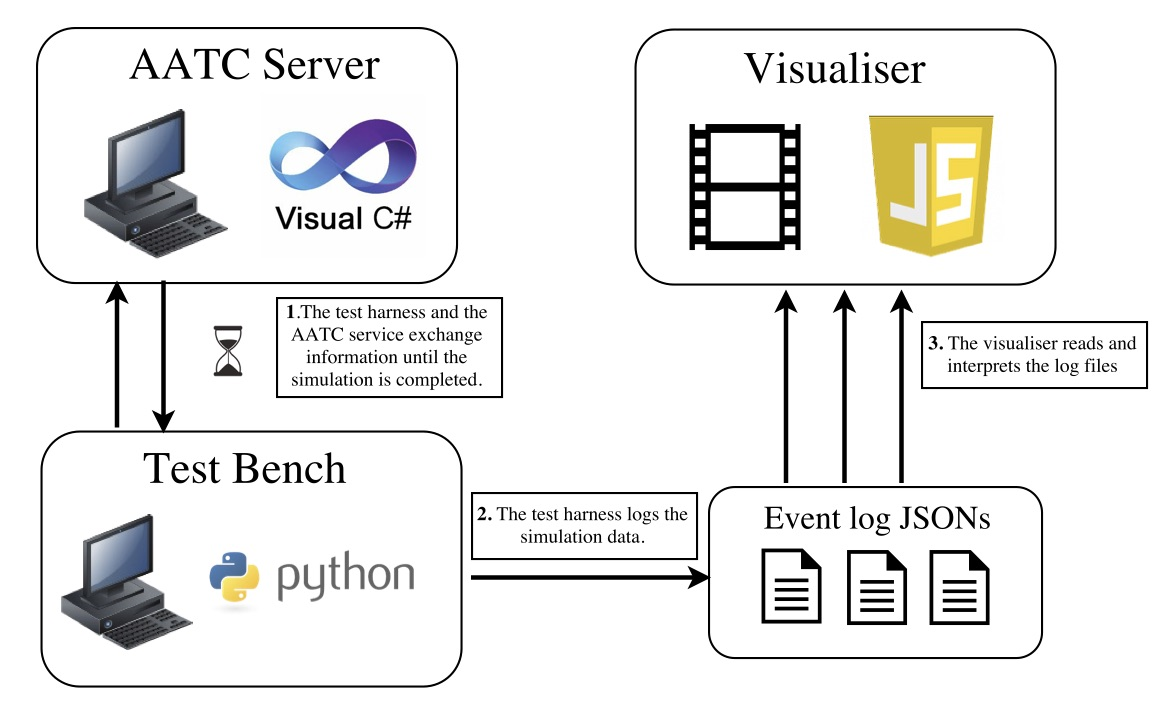
\includegraphics[width=0.8\linewidth]{img/aatc_tech_overview.jpg}
  \caption{Technical Overview of AATC. \cite{Balaji2017}}
  \label{fig:aatc_tech_overview}
\end{figure}

The system was designed with three challenges in mind. The first challenge was to route drones from their origins to their destinations, and secondly, to ensure they avoided collisions with both static and dynamic obstacles - such as the ones mentioned in Section 2.1. The last challenge is to design the system in such a way that it would be able to scale to hundreds and thousands of drones. \\

To this end, a \textit{Global Layer} was built to deal with static obstacles (such as NFZs) by calculating a path for the drone around NFZs before it begins its journey. The second problem was tackled with a \textit{Reactive Layer} that handles non-static obstacles (such as manned aviation and other drones). This is the layer that would be providing the real-time updates to drones as they poll the server every second. \\

Only one drone type was used in AATC, with its specification outlined in Figure \ref{fig:edrone}. It has a radius of 1m and a maximum velocity in any direction of 5 metres per second.

\begin{figure}[!hbpt]
  \center
  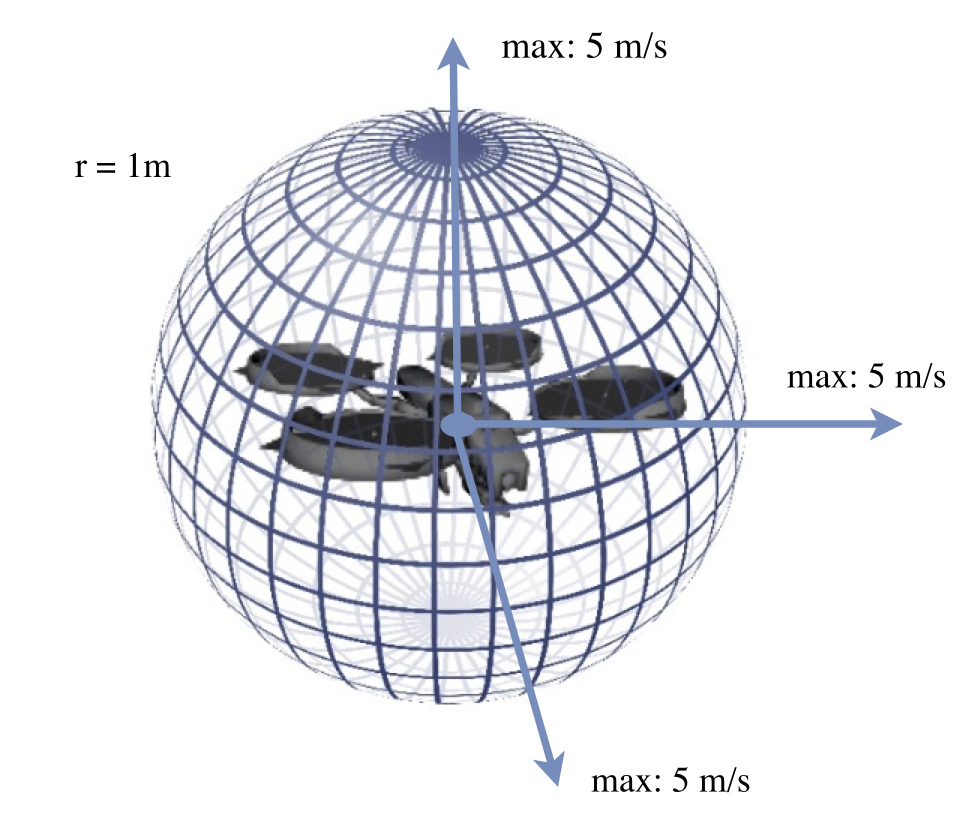
\includegraphics[width=0.4\linewidth]{img/edrone.jpg}
  \caption{The default AATC drone model. \cite{Balaji2017}}
  \label{fig:edrone}
\end{figure}

\subsection{The Global Layer}
The Global Layer holds the static representation of the world so that given a start and end, it can compute an optimal set of waypoints that a drone should follow - thereby dealing with AATC's path-finding problem.

\subsubsection{Dijkstra's Algorithm}
Dijkstra's algorithm is a popular algorithm to find the shortest paths between nodes in a graph. When using a co-ordinate grid system, each coordinate could represent a node in a graph and thus the algorithm can also be used to find the shortest path between a source and destination. Appendix A is an example implementation of Dijkstra in Python. \\

However, in the real world, we also have to consider the cost of computation and potentially make use of heuristics in order to return the shortest path given a limited amount of time. Especially in the drone case, we want to compute a good path as quick as possible in order to let the drone proceed along its way.

\subsubsection{A* Algorithm}
Enter, the A* algorithm. This algorithm is a generalisation of Dijkstra's algorithm that reduces the number of nodes explored during the search process by use of a heuristic - typically a minimum distance to the destination. A benefit over Dijkstra in particular is that it considers the distance already traveled into account, which aids the heuristic mechanism. \\

Naturally, by searching less nodes on a graph, less computation is performed and therefore A* has better performance than just using a pure form of Dijkstra's algorithm.

\begin{figure}[!hbpt]
  \center
  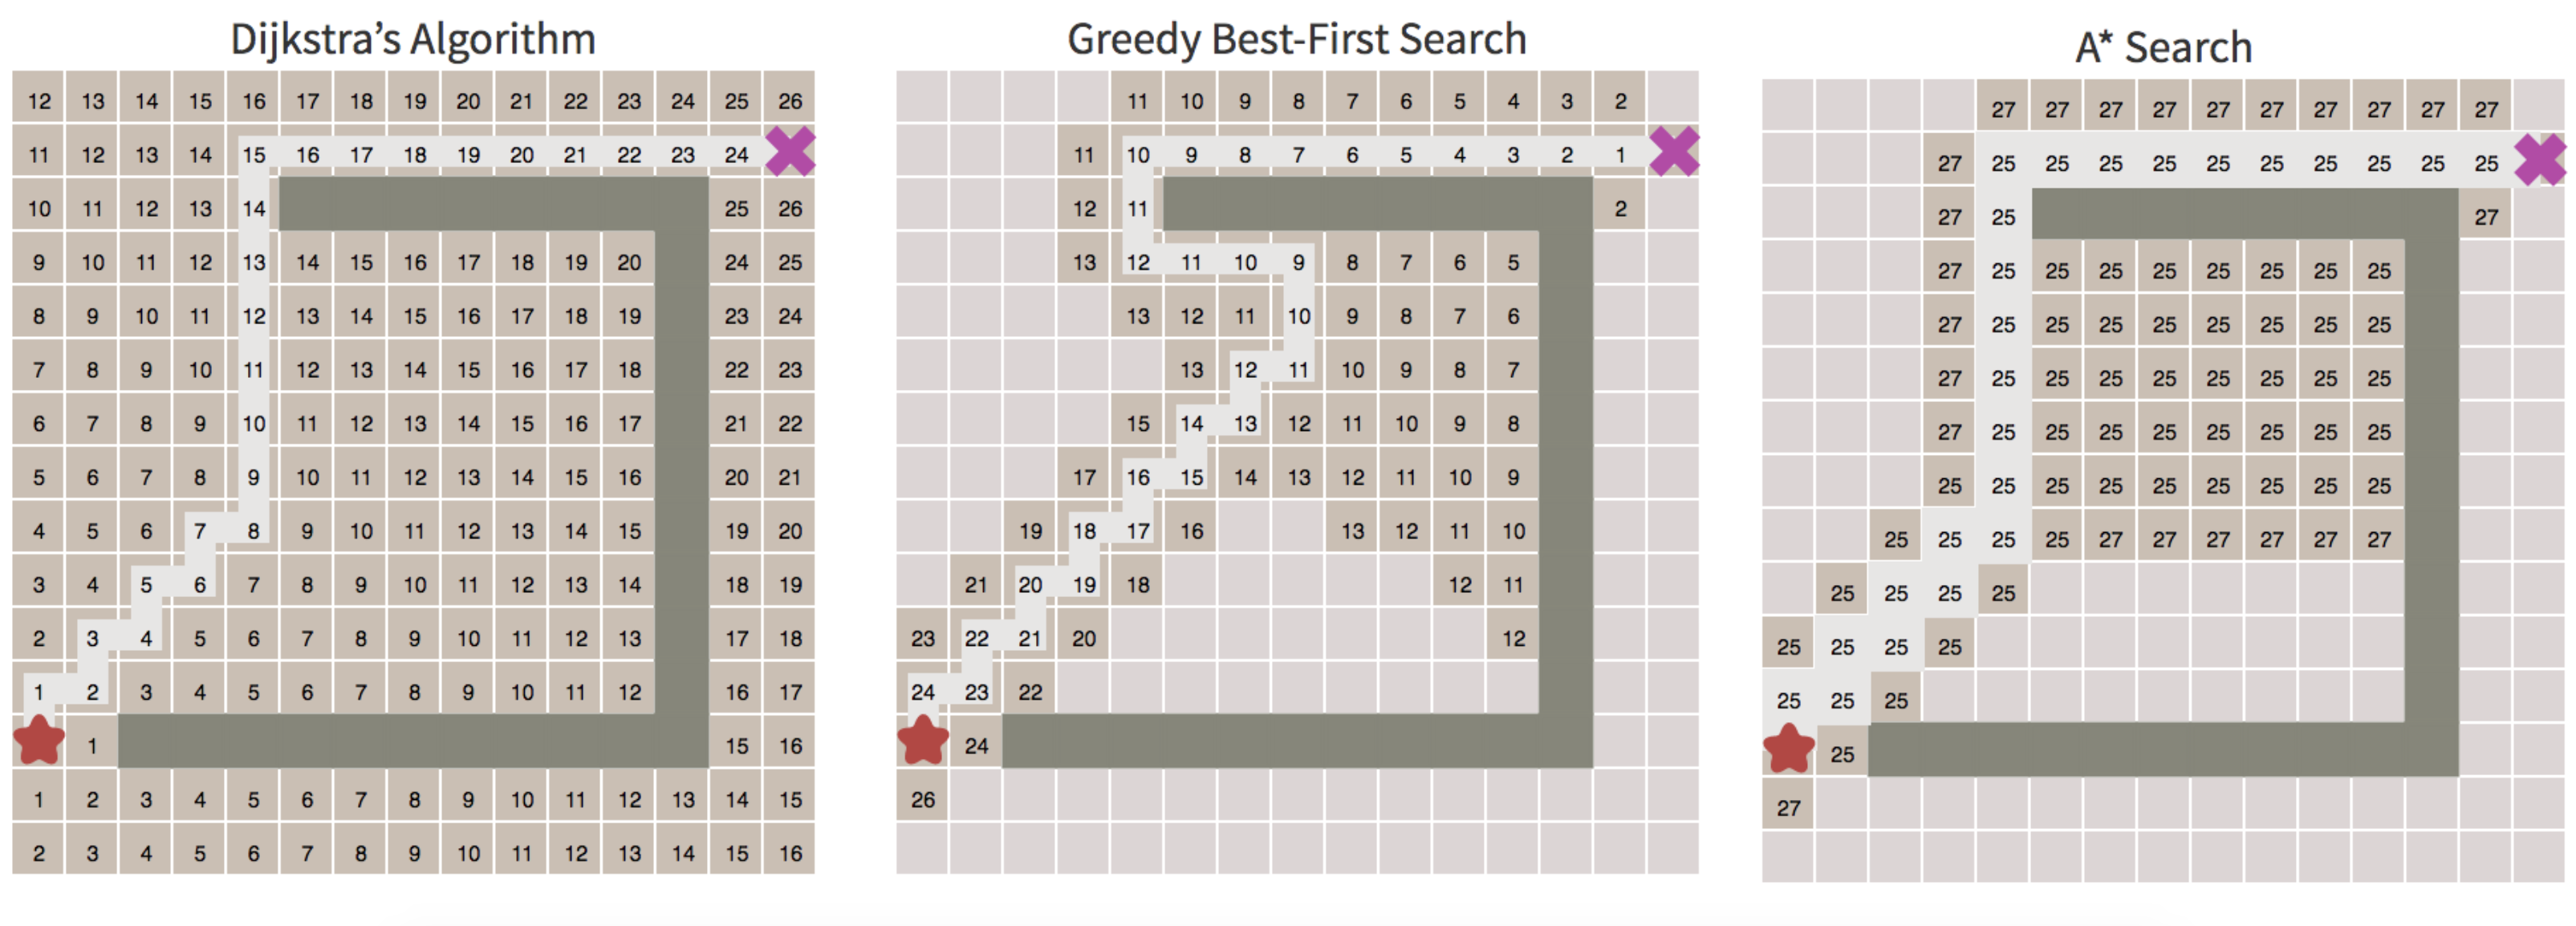
\includegraphics[width=\linewidth]{img/search_comparison.png}
  \caption{Comparing popular search algorithms. \cite{Balaji2017}}
  \label{fig:search_comparison}
\end{figure}

But for all these positive aspects, one must remember that our use for this algorithm is to compute paths in a real world, which is not necessarily split up into a nice, clean grid. So we turn our attention to a modification of the A* algorithm: Theta*.

\subsubsection{Theta* Algorithm}
The Theta* algorithm is an any-angle pathfinding algorithm based on the A* algorithm that introduces Line of Sight (LOS) checks, which means that each jump from node to node in the returned path can be at any angle and not just up, down, left or right. This neat addition allows Theta* to be capable of finding near-optimal paths with a runtime comparable to A* \cite{Uras2015}. \\

\begin{figure}[!hbpt]
  \center
  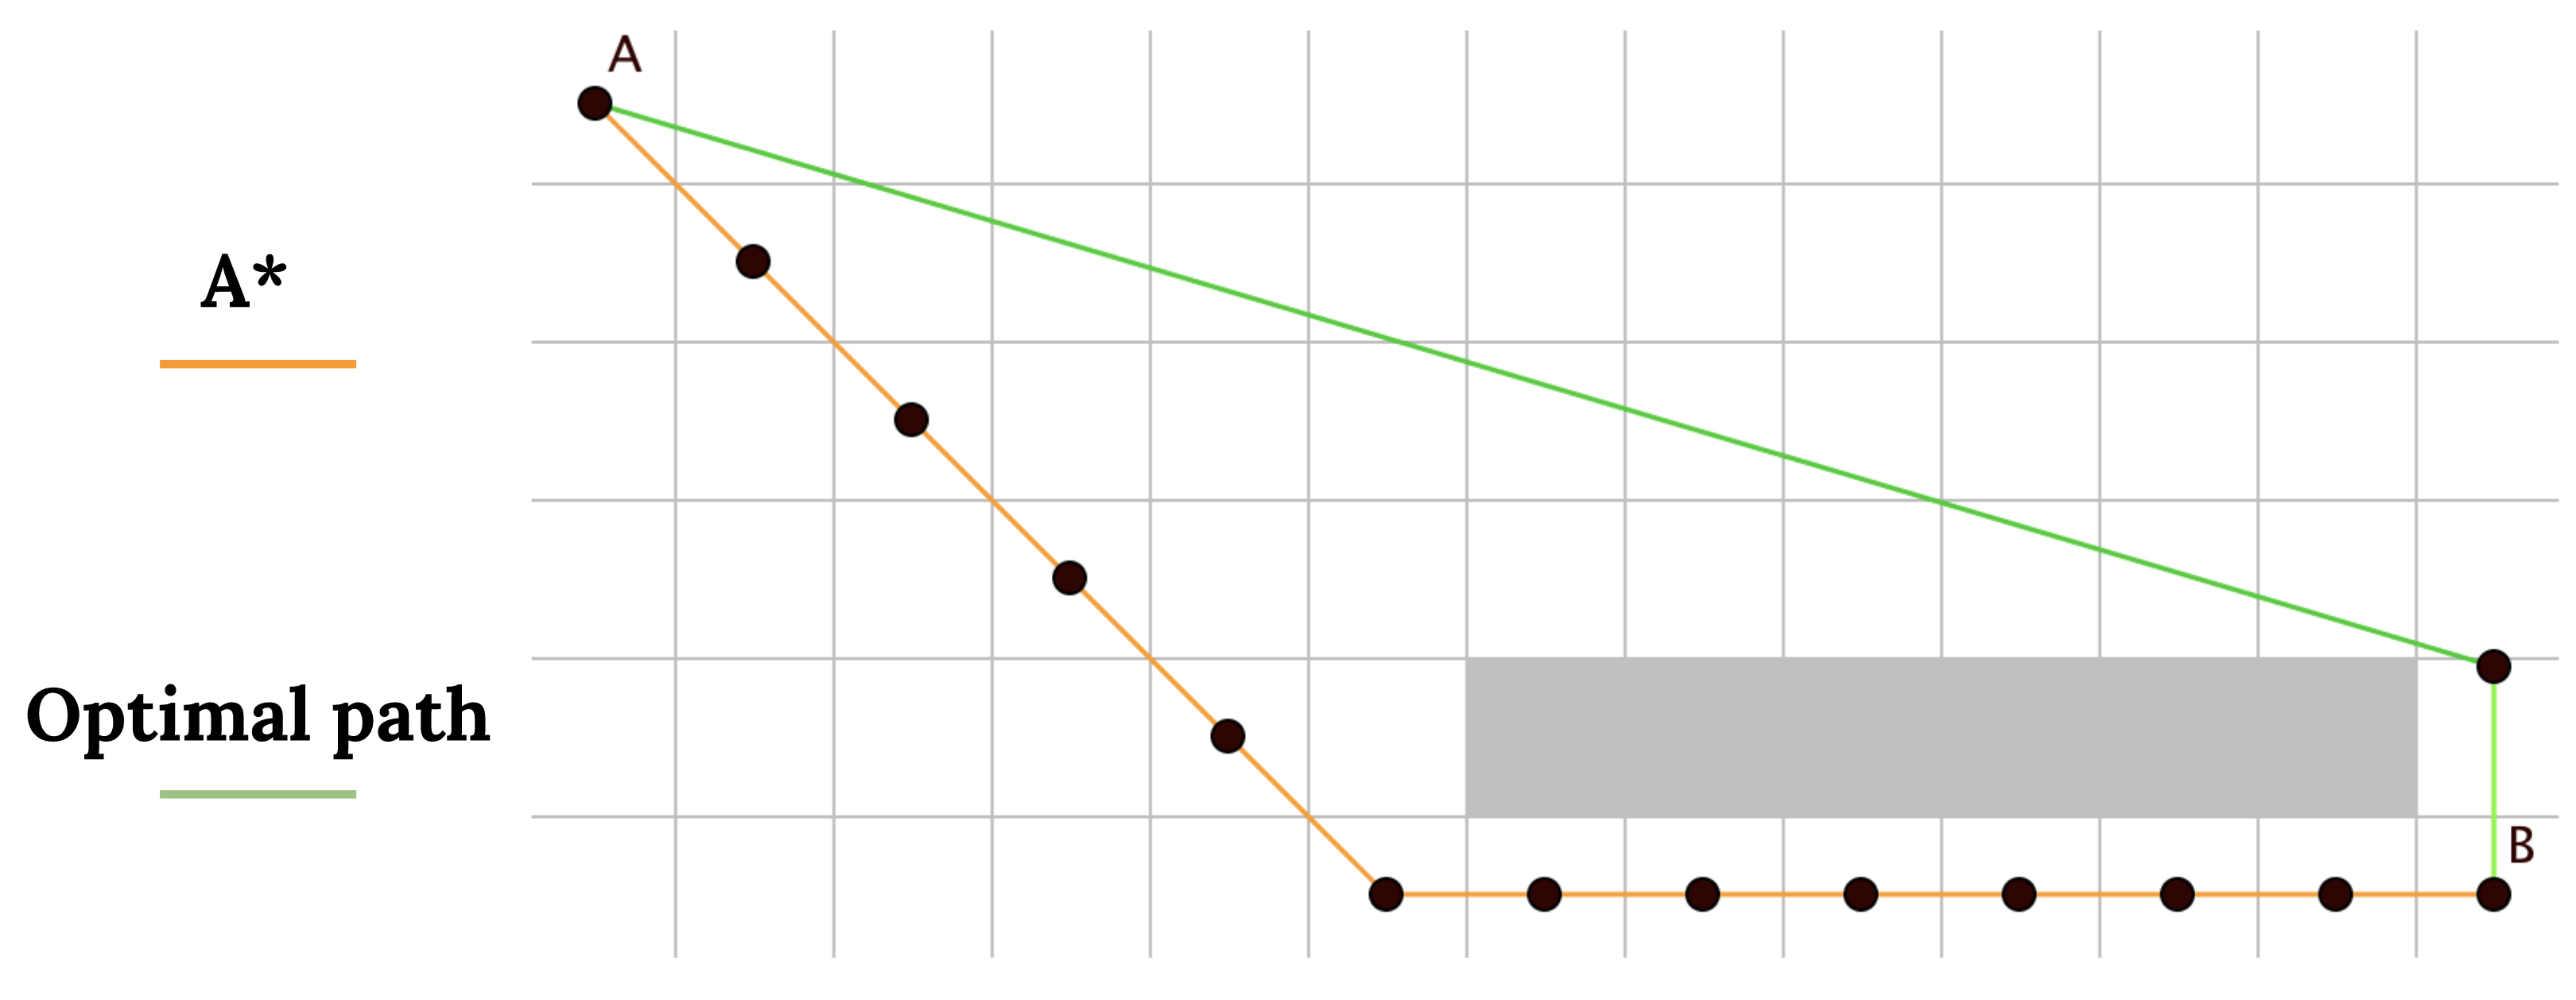
\includegraphics[width=\linewidth]{img/a_star_vs_optimal.png}
  \caption{A* VS Optimal Path. \cite{Balaji2017}}
  \label{fig:a_star_vs_optimal}
\end{figure}

Being able to get as short a path as possible is absolutely vital in the drone use-case because they have limited flying time. After all, their batteries can only last so long before they need to be recharged. Therefore, it is important to ensure drones travel as little distance as possible in order to maximise the number of times they can be used between charges.

\subsubsection{Lazy Theta* Algorithm}
A further optimisation is to reduce the number of LOS checks performed, as found in another paper by the original authors of the Theta* algorithm\cite{Nash2010}. This algorithm assumes every node is in line of sight of its parent, and the LOS check is only performed once the child node is expanded on. If this turns out to be false, then the algorithm defaults to a typical A* approach. Reducing the number of LOS checks therefore improves the algorithm's overall performance.

\subsubsection{Conclusions}
As seen on Table \ref{tab:aatc_exec_time}, A* has far better execution times than both Theta* variants but when we get to Table \ref{tab:aatc_total_drone_distance} it is evident that Lazy/Theta* produces better paths because the total distance travelled by drones is fewer. Therefore, Lazy Theta* was chosen as the core algorithm for the Global Layer.

\begin{table}[!hbpt]
\centering
\begin{tabular}{|l|c|c|}
\hline
\multicolumn{1}{|c|}{Test Case} & A* & \multicolumn{1}{l|}{Theta* and Lazy Theta Star} \\ \hline
Queen Threat & 6.11 & 5.98 \\ \hline
The Imperial Tunnel & 10.83 & 10.22 \\ \hline
The Great London Beehive & 52.63 & 49.77 \\ \hline
The Nightmare of Hyde Park & 118.4 & 115.32 \\ \hline
The Great Wall of Imperial College & 16.37 & 15.46 \\ \hline
Multi Drone collision & 15.27 & 14.82 \\ \hline
\end{tabular}
\caption{Total path distances for all drones (in km). \cite{Balaji2017}}
\label{tab:aatc_total_drone_distance}
\end{table}

\begin{table}[!hbpt]
\centering
\begin{tabular}{|c|c|c|c|}
\hline
Test Case                          & A*                                                          & \multicolumn{1}{l|}{Theta*}                                   & \multicolumn{1}{l|}{Lazy Theta*}                              \\ \hline
Imperial Tunnel                    & \begin{tabular}[c]{@{}c@{}}118\\ 120\\ 121\end{tabular}     & \begin{tabular}[c]{@{}c@{}}141\\ 138\\ 137\end{tabular}       & \begin{tabular}[c]{@{}c@{}}124\\ 132\\ 129\end{tabular}       \\ \hline
Imperial Tunnel Mean               & 119.7                                                       & 138.7                                                         & 128.3                                                         \\ \hline
The Great London Beehive (GLB)           & \begin{tabular}[c]{@{}c@{}}859\\ 916\\ 894\end{tabular}     & \begin{tabular}[c]{@{}c@{}}1318\\ 1486\\ 1555\end{tabular}    & \begin{tabular}[c]{@{}c@{}}1166\\ 1075\\ 1201\end{tabular}    \\ \hline
The GLB Mean                       & 889.7                                                       & 1453                                                          & 1147.4                                                        \\ \hline
The Nightmare of Hyde Park (NHP)        & \begin{tabular}[c]{@{}c@{}}9771\\ 9687\\ 10118\end{tabular} & \begin{tabular}[c]{@{}c@{}}28436\\ 27970\\ 28273\end{tabular} & \begin{tabular}[c]{@{}c@{}}21330\\ 24786\\ 21609\end{tabular} \\ \hline
The NHP Mean                       & \multicolumn{1}{l|}{9858.7}                                 & \multicolumn{1}{l|}{28226.4}                                  & 22575                                                         \\ \hline
The Great Wall Of Imperial College (GWIC) & \begin{tabular}[c]{@{}c@{}}394\\ 447\\ 416\end{tabular}     & \begin{tabular}[c]{@{}c@{}}913\\ 910\\ 912\end{tabular}       & \begin{tabular}[c]{@{}c@{}}838\\ 840\\ 841\end{tabular}       \\ \hline
The GWIC Mean                      & 419                                                         & 911.7                                                         & 839.7                                                         \\ \hline
\end{tabular}
\caption{Execution times for pathfinding algorithms on AATC test cases. \cite{Balaji2017}}
\label{tab:aatc_exec_time}
\end{table}

\newpage
\subsection{The Reactive Layer}
Given the list of waypoints that the Global Layer generates, the Reactive Layer's task is to provide the right speed and direction to drones whilst taking into consideration any dynamic obstacles that the drone may face, such as manned aviation, other drones and potentially dynamic NFZs.

\subsubsection{Artificial Potential Fields (APF)}
A novel way to approach this layer is to create an Artificial Potential Field (APF) in the area the drone operates in, and give each point in this field a potential\cite{Zhu2016}. By having a low potential for the destination and large potentials at obstacles, the drone simply has to move in a way to get to point of lowest potential. It is analogous to a magnet in a magnetic field, repelled by obstacles and attracted to its destination. \\

Although one might argue that the Global Layer is not needed anymore because the Reactive Layer solves the pathfinding problem, there are a few issues that arise with this idea. As Figure \ref{fig:apf_comp} shows, a U-shaped object poses a problem because the drone may be attracted to the destination and then quickly repelled by the obstacle, and then back to being attracted - and this cycle is seemingly endless.

\begin{figure}[!hbpt]
  \center
  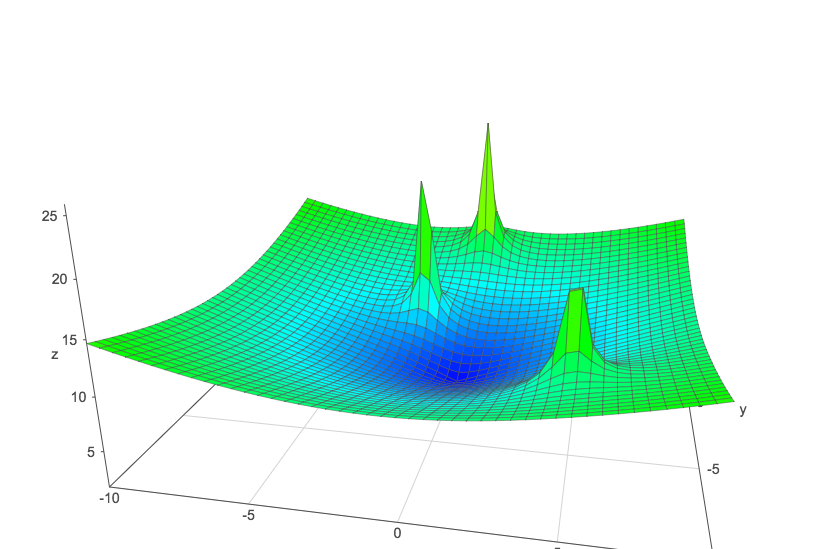
\includegraphics[width=0.9\linewidth]{img/obst.png}
  \caption{APF with obstacles (green peaks) and a destination (blue trough). \cite{Balaji2017}}
  \label{fig:obst}
\end{figure}

By introducing a random element, as in Rotating APF, the object is repelled in a slightly different direction each time to make it out of the trap and eventually reach its destination. Even this method, however, does not actually guarantee that the drone makes it past the U-shaped obstacle because it depends on how the random element behaves and also whether the drone has enough battery to be loitering for long.

\begin{figure}[!hbpt]
  \center
  \includegraphics[width=\linewidth]{img/apf_comp.png}
  \caption{Pure APF vs Rotating APF vs AATC Implementation. \cite{Balaji2017}}
  \label{fig:apf_comp}
\end{figure}

Clearly, integrating both layers proves most fruitful - as the waypoints generated by the Global Layer are used to quite literally navigate around the problematic aspects of the Reactive Layer. This integration that was implemented in the AATC project.

\subsubsection{Equations for APF}
The full set of equations used to obtain the recommended unnormalized velocity $v_{raw}$ of the drone is:
$$U_a = \rho_ad_{goal}$$
$$U_r =  \begin{cases}
      \rho_r\frac{1}{d_{obst} - d_{safe}} & d_{obst} \leq d_{influence}   \\
      0 & otherwise \\

   \end{cases}
$$
$$U_{ret} = \rho_{ret}d_{last}$$
$$U = U_a + U_r + U_{ret}$$
$$\bm{v_{raw}} = \nabla U$$

where $\nabla U$ is the gradient of U, and U is the magnitude of potential at a point\cite{Balaji2017}.

Since $\nabla U$ is the recommended velocity, it can be computed from first principles:
$$\nabla U(x,y,z) = \colvec{3}
                {\frac{\delta U(x,y,z)}{\delta x}}
                {\frac{\delta U(x,y,z)}{\delta y}}
                {\frac{\delta U(x,y,z)}{\delta z}}
                  \approx \colvec{3}
                {U(x + 1,y,z) -  U(x,y,z)}
                {U(x,y + 1,z) -  U(x,y,z)}
                {U(x,y,z + 1) -  U(x,y,z)}$$

The recommended velocity can now be computed by first calculating the potential at 4 points. To calculate the potential at a given point, one must find the sum of:
\begin{itemize}
  \item $U_a$ - attraction potential using euclidean distance to next waypoint.
  \item $U_r$ - repulsion potential using euclidean distance to nearest obstacle.
  \item $U_{ret}$ - return potential using euclidean distance to point from last time step.
\end{itemize}

To allow drones to gently come to their goals instead of shooting past and potentially missing, the recommended speed is calculated by taking the minimum of the drone's max speed and the distance to the goal:
$$ speed = min(max\_speed, d_{goal}) $$

The gradient $\nabla U$ is then normalised to be a unit vector before being multiplied by the speed to compute the final velocity.

\subsubsection{Genetic Algorithm}
By paying close attention to Section 2.4.2, we can identify several undefined constants: $\rho_r$, $\rho_a$, $\rho_{ret}$ and $d_{influence}$. The balance between them is key, because if $\rho_a$ is too high relative to $\rho_r$ then the drones ignore obstacles and die on impact, but if $\rho_r$ is too high then they will oscillate between objects and never reach their goal. After much fiddling about with "magic numbers", a genetic algorithm was employed to provide the optimal values for the specific drone model. \\

Genetic algorithms are a metaheuristic inspired by the process of natural selection, and they are a way by which high-quality solutions can be generated for optimisation problems\cite{Mitchell1996}. In the case of AATC, the aforementioned constants need to be fine-tuned in order to produce an APF model that, to its best ability, does not return absurd, erroneous velocities. See Figure \ref{fig:aatc_spaghett} as an example. \\

\begin{figure}[!hbpt]
  \center
  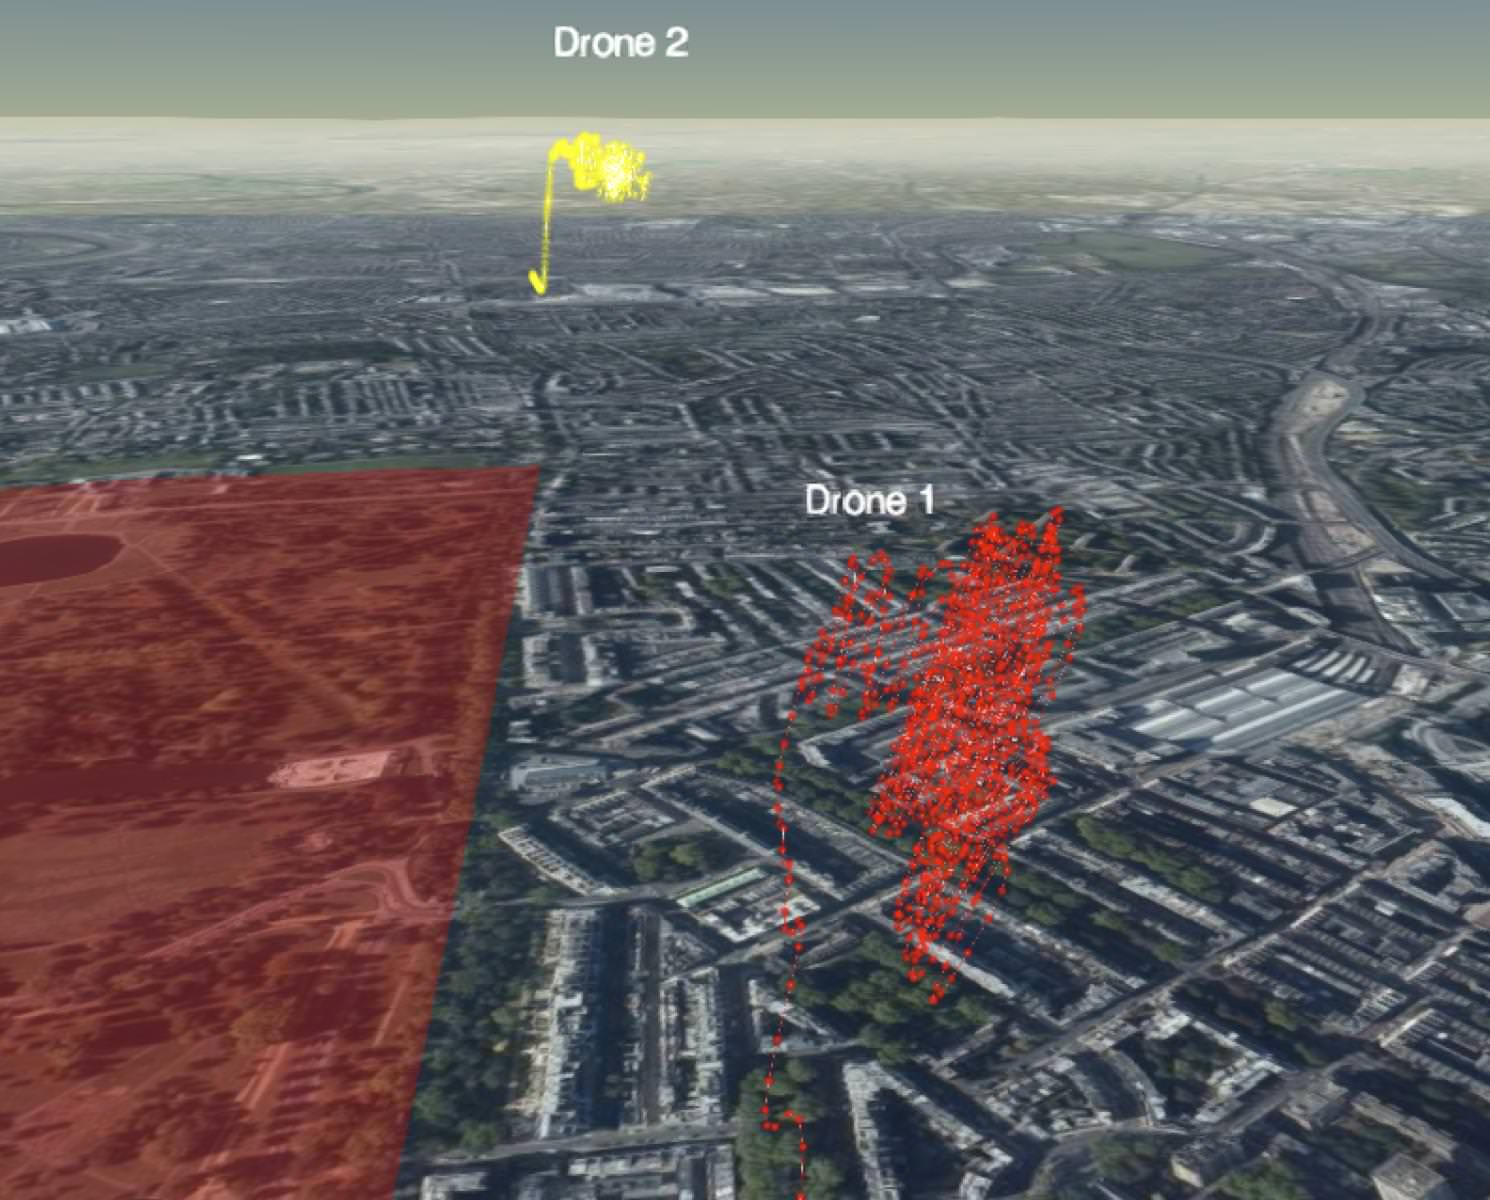
\includegraphics[width=\linewidth]{img/aatc_spaghett.jpg}
  \caption{Drone paths after increasing repulsion constant by 3 orders of magnitude.}
  \label{fig:aatc_spaghett}
\end{figure}

Effectively, an initial range of values (see Table \ref{tab:gen_alg}) is provided and the genetic algorithm cycles through all of these, letting these constants compete against each other to see which set of constants produces the simulation with the lowest cost. This cost is determined from a cost function that returns the remaining battery life of a drone if it reaches its destination, or a relatively huge number otherwise.
$$cost = \sum_{testcase} \sum_{drone}
    \begin{cases}
      batteryUsed & if \; drone \; reached \; destination    \\
      100000 & otherwise \\

   \end{cases}$$

\begin{table}[!hbpt]
\centering
\begin{tabular}{|l|l|l|l|l|}
\hline
Constant           & Min & Max & Step & Total \\ \hline
Attraction         & 0.8 & 1.1 & 0.1    & 3     \\ \hline
Repulsion          & 100 & 500 & 100  & 5     \\ \hline
Return             & 0.1 & 0.7 & 0.2  & 4     \\ \hline
Influence distance & 300 & 600 & 100  & 4     \\ \hline
\multicolumn{4}{|l|}{Population}      & 240   \\ \hline
\end{tabular}
\caption{Initial configuration of the genetic algorithm for AATC. \cite{Balaji2017}}
\label{tab:gen_alg}
\end{table}

\subsubsection{Conclusions}
In the end, the genetic algorithms only improved the simulations by about 2\%\cite{Balaji2017} which could mean that the original range of constants was already a good set to work with. However, there is still scope for even greater improvements if the genetic algorithm was to be run with a greater number of test scenarios, bigger range of values to cycle through, and generally larger simulations.

\subsection{Delivery Networks}
From the ancient days of Assyrian trade in 19 BCE \cite{stearns2001the}, to the modern day online market - the ability to trade goods and services has had a profound impact on the way we live our lives. Thanks to globalisation and the explosion of the internet, we are now able to use a service such as Amazon Prime and get goods delivered within days, if not hours, of purchasing through a simple click. Through it all, physical delivery networks enable this online retail behemoth.



\subsubsection{Planes}
\subsubsection{Trucks}
\subsubsection{Drones}

\subsection{Prioritising Economic Value}
% Thus far, we have shown that whilst there is great scope to utilise drones for delivery of physical goods, AATC technology only touches upon the routing aspect - how to get from point A to point B. In all the test cases, the drones' start and end points were hand-picked by the developers\cite{Balaji2017} to give an insight into how AATC would operate in a variety of scenarios.


\subsubsection{Quality of Service}
\subsubsection{Value Curve}
\subsubsection{skdbsa}

\subsection{SpatialOS}
\subsubsection{Unity SDK}
\subsubsection{Layered Simulation}
\subsubsection{Distributed Simulation}
Example text 1\\

Example text 2\\

Example text 3

%**********************************************%
\newpage
\section{Project Plan}
\subsection{Phase 1: Porting Global and Reactive Layers to SpatialOS}
\subsection{Phase 2: Implementing a Scheduling Layer}
\subsection{Phase 3: Visualising the Economic Value}
\subsection{Stretch Goals}

%**********************************************%
\newpage
\section{Evaluation Plan}

%**********************************************%
%\newpage
%\section{Conclusion \& Future Work}
%blabla

%**********************************************%
\newpage
\addcontentsline{toc}{section}{References}

\bibliography{library}
\bibliographystyle{abbrv}

\newpage

\begin{appendices}
\section{Python Implementation of Dijkstra's Algorithm}
\begin{lstlisting}[language=Python, caption=Example Implementation from GitHub. \cite{Root}]
def dijsktra(graph, initial):
  visited = {initial: 0}
  path = {}

  nodes = set(graph.nodes)

  while nodes:
    min_node = None
    for node in nodes:
      if node in visited:
        if min_node is None:
          min_node = node
        elif visited[node] < visited[min_node]:
          min_node = node

    if min_node is None:
      break

    nodes.remove(min_node)
    current_weight = visited[min_node]

    for edge in graph.edges[min_node]:
      weight = current_weight + graph.distance[(min_node, edge)]
      if edge not in visited or weight < visited[edge]:
        visited[edge] = weight
        path[edge] = min_node

  return visited, path
\end{lstlisting}

\end{appendices}

\end{document}
